\documentclass[final]{article}
\usepackage{bm}
\usepackage{amsmath}
\usepackage{amssymb}
\usepackage{hyperref}
\usepackage{rotating}
\usepackage{float}
\usepackage{graphicx}
\usepackage{wrapfig}
\usepackage{subcaption}
\usepackage{amsmath, mathtools}
\usepackage{listings}
\usepackage{color}
\usepackage[extrafootnotefeatures, Kashida]{xepersian}
\usepackage{multirow}
\usepackage{fourier}
\settextfont{XB Niloofar}
\setdigitfont{XB Niloofar}
\hypersetup{
	colorlinks=true,
	linkcolor=blue,
	filecolor=blue,      
	urlcolor=cyan,
}
\definecolor{dkgreen}{rgb}{0,0.6,0}
\definecolor{gray}{rgb}{0.5,0.5,0.5}
\definecolor{mauve}{rgb}{0.58,0,0.82}
\definecolor{apricot}{rgb}{0.98046, 0.894,0.8014}
\lstset{ %
	language=R,                     % the language of the code
	basicstyle=\footnotesize,       % the size of the fonts that are used for the code
	numbers=left,                   % where to put the line-numbers
	numberstyle=\tiny\color{gray},  % the style that is used for the line-numbers
	stepnumber=1,                   % the step between two line-numbers. If it's 1, each line
	% will be numbered
	numbersep=5pt,                  % how far the line-numbers are from the code
	backgroundcolor=\color{apricot},  % choose the background color. You must add \usepackage{color}
	showspaces=false,               % show spaces adding particular underscores
	showstringspaces=false,         % underline spaces within strings
	showtabs=false,                 % show tabs within strings adding particular underscores
	frame=single,                   % adds a frame around the code
	rulecolor=\color{black},        % if not set, the frame-color may be changed on line-breaks within not-black text (e.g. commens (green here))
	tabsize=2,                      % sets default tabsize to 2 spaces
	captionpos=b,                   % sets the caption-position to bottom
	breaklines=true,                % sets automatic line breaking
	breakatwhitespace=false,        % sets if automatic breaks should only happen at whitespace
	title=\lstname,                 % show the filename of files included with \lstinputlisting;
	% also try caption instead of title
	keywordstyle=\color{blue},      % keyword style
	commentstyle=\color{dkgreen},   % comment style
	stringstyle=\color{dkgreen},      % string literal style
	escapeinside={\%*}{*)},         % if you want to add a comment within your code
	morekeywords={*,...}            % if you want to add more keywords to the set
} 
\def\ojoin{\setbox0=\hbox{$\bowtie$}%
	\rule[-.02ex]{.25em}{.4pt}\llap{\rule[\ht0]{.25em}{.4pt}}}
\def\leftouterjoin{\mathbin{\ojoin\mkern-5.8mu\bowtie}}
\def\rightouterjoin{\mathbin{\bowtie\mkern-5.8mu\ojoin}}
\def\fullouterjoin{\mathbin{\ojoin\mkern-5.8mu\bowtie\mkern-5.8mu\ojoin}}


%\makeatletter
%\renewcommand{\thesection}{%
%  \ifnum\c@chapter<1 \@arabic\c@section
%  \else \thechapter.\@arabic\c@section
%  \fi
%}
%\makeatother

\title{
طراحی سیستم‌های دیجیتال
	\\
	{
		\large
		گزارش نهایی پروژه‌ی سوم
	}
}
\author{
	\begin{tabular}{rl}
		مهبد مجید	&
		۹۵۱۰۹۳۷۲
		\\
		سبحان محمدپور & 
		۹۵۱۰۶۶۰۷
		\\
		کیمیا حمیدیه &
		۹۵۱۰۹434
		\\
		روژین نوبهاری
		&
		۹۵۱۰۵۲۳۸
		\\
		کوشا جافریان
		&
		۹۵۱۰۵۴۵۴
	\end{tabular}
}

\begin{document}
	\maketitle
	
	\section*{توصیف اولیه}
\subsection*{مقدمه}
امروزه با توجه به کاربرد گسترده‌ی
\lr{Java}
و بالطبع
\lr{JVM}
،
در صنعت و جهان مدرن امروزی منطقی به نظر می‌رسد که فرآیند اجرای کدهای جاوا را سریع‌تر کنیم.
یکی از راه‌های خوب برای رسیدن به این مهم، می‌تواند پیاده‌سازی سخت‌افزاری 
\lr{JVM}
که در واقع هسته‌ی جاواست  باشد.
\subsection*{اهداف}
در این پروژه می‌خواهیم برای پردازنده‌ی 
\lr{ARM-7}(صبای ۲)
یک شتاب‌دهنده‌
\LTRfootnote{accelerator}
‌ی سخت‌افزاری
\lr{JVM}
بسازیم.
نحوه‌ی کار این شتاب‌دهنده به این شکل است که پردازنده 
\lr{opcode}های
\lr{JVM}
را دریافت می‌کند و به شتاب‌دهنده می‌دهد و شتاب‌دهنده دستورات معادل پردازنده را تولید می‌کند.
\subsection*{مراحل انجام پروژه}
به طور کلی با توجه به اهداف پروژه ما باید ۳ کار را برای انجام پروژه انجام‌دهیم:
\begin{itemize}
	\item 
	یادگیری کار با ماشین
	\lr{JVM}
	\item
	یادگیری کار با ماشین
	\lr{ARM-7}
	\item
	ساخت مبدل برای تبدیل دستورات میان این دو
\end{itemize}
	
	\section*{تقسیم‌بندی پروژه}
\subsection*{انتخاب
	\lr{opcode}ها}
ابتدا لیست
\lr{opcode}های
\lr{JVM}
را پیداکردیم. از آنجایی که قرار بود این پروژه برای ۵ تیم باشد، نیاز بود تا تعدادی از آپکدها را جداکنیم که پروژه برای ۴ تیم مناسب شود.
برای جداکردن تعدادی از این
\lr{opcode}ها
از
\lr{Jazelle}
الگو می‌گیریم. 
\lr{Jazelle}
به این صورت عمل می‌کند که
\lr{JVM}
دستوراتش را به
\lr{Jazelle}
می‌فرستد و اگر
\lr{Jazelle}
از آن‌ها پشتیبانی کرد، آن‌ها را اجرا می‌کند، و اگر هم پشتیبانی نمی‌کرد آن‌ها را به
\lr{JVM}
باز می‌گرداند تا آن‌ها را به دستوراتی که
\lr{Jazelle}
از آن‌ها پشتیبانی می‌کند تبدیل کند.
\begin{figure}[H]
	\centering
	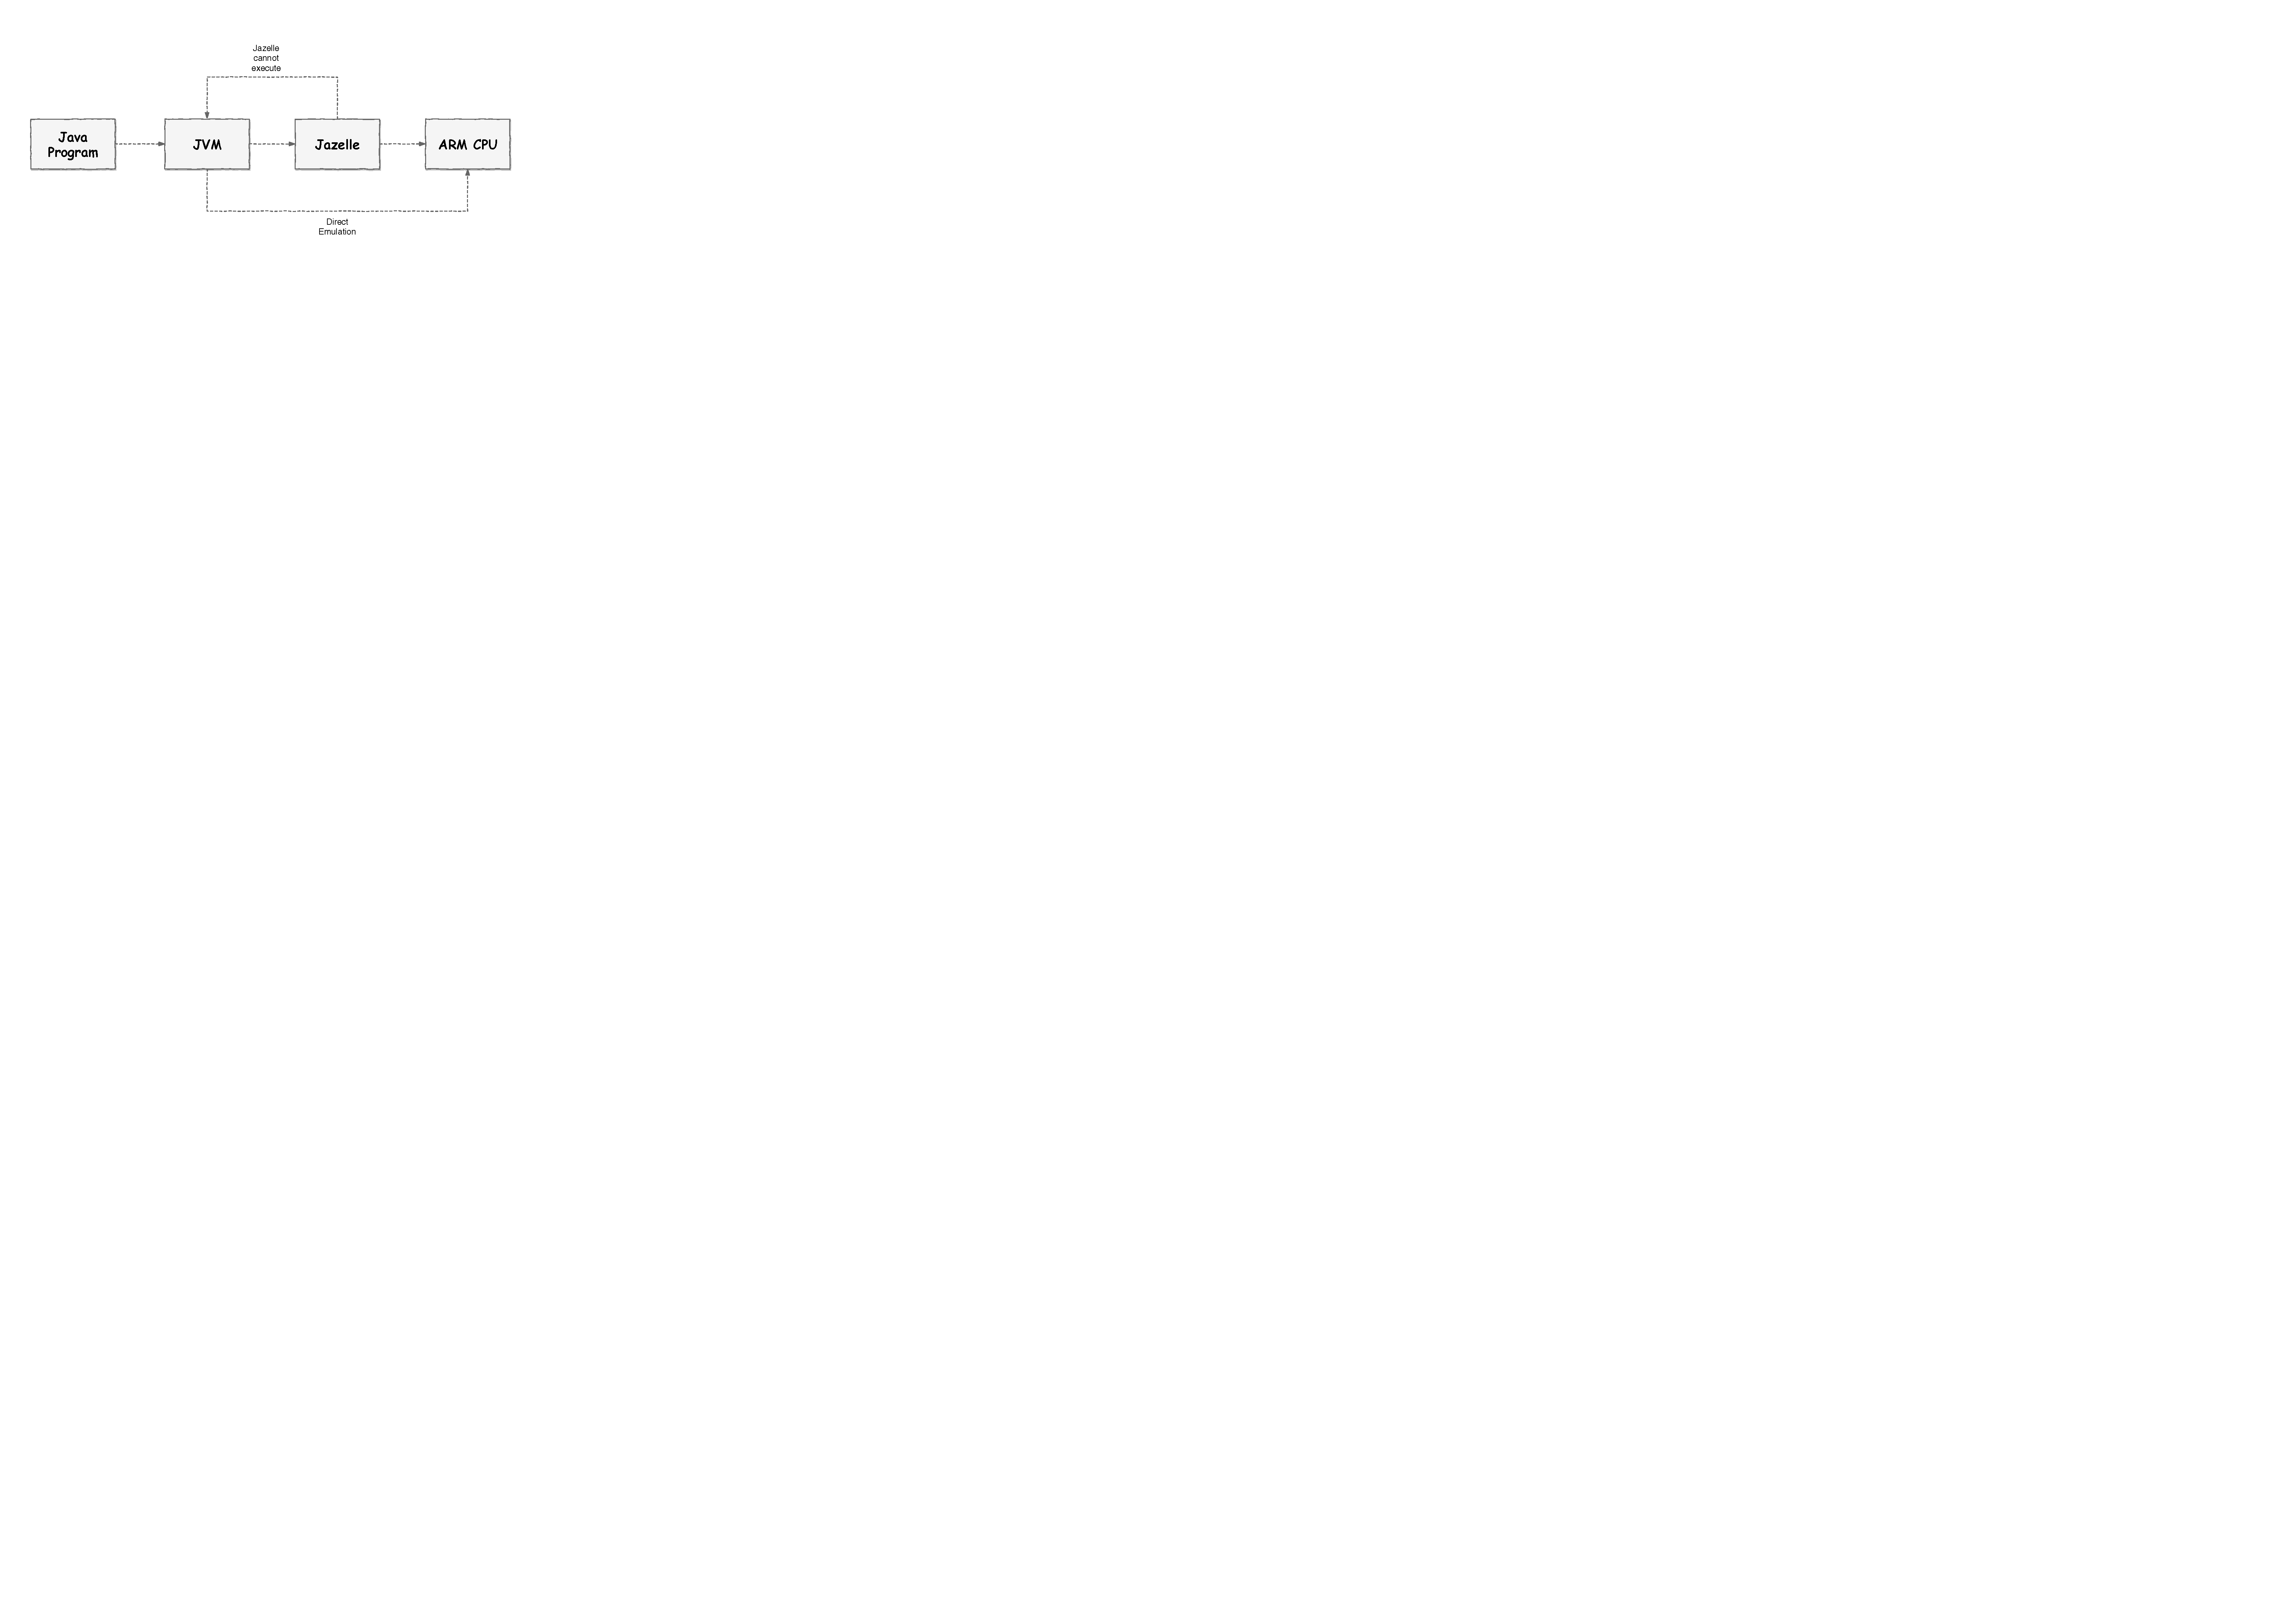
\includegraphics[width=\linewidth]{flowchart}
	\caption{روند اجرای کار jazelle}
	\label{fig:flowchart}
\end{figure}

ما نیز به این صورت عمل می‌کنیم که عده‌ای از 
\lr{opcode}ها
که پیاده‌سازی نرم‌افزاریشان ساده‌تر است را جدا می‌کنیم و الباقی
\lr{opcode}ها 
را در پیاده‌سازیمان می‌آوریم.
\subsection*{تقسیم‌بندی 
	\lr{opcode}ها
}
برای افزایش بازدهی گروه‌ها
\lr{opcode}های
انتخابی به شانزده بسته‌ی ۱۰تایی تقسیم‌بندی شدند و با یک کد 
\lr{R}
که به صورت رندوم این ۱۶ بسته را به گروه‌ها تخصیص می‌داد، تقسیم‌بندی کردیم.(سید را هم با حضور اعضای سایر گروه‌ها تعیین‌کردیم.)
\subsubsection*{کد}
\begin{latin}
	\begin{lstlisting}
	library(dplyr)
	set.seed(1919)
	s = sample(seq(from = 1, to = 16), replace = F)  
	c("jaferian", "asadi", "hoseini", "ghafarloo") %>% 
	cbind(t(apply(matrix(s, nrow = 4), 1, sort)))
	\end{lstlisting}
\end{latin}
\subsubsection*{خروجی کد}
\begin{latin}
	\centering
	\begin{tabular}{l|cccc}
		Group Name & & & & \\
		\hline \hline
		jaferian & 4 & 6 & 7 & 8\\
		
		asadi & 3 & 9 & 10 & 12\\
		hoseini & 1 & 5 & 11 & 14\\
		ghafarloo & 2 & 13 & 15 & 16\\
	\end{tabular}
\end{latin}
\subsubsection*{لیست دستورات}
لیست دستورات را می‌توانید در صفحه‌گسترده‌ی ۱ و ۲ مشاهده‌کنید.


	\section*{
	برخی ]dماژول‌های پیاده‌سازی‌شده با
	\lr{verilog}
}

\subsection*{فایل 
	\lr{memory.v}
}
در این فایل دو ماژول حافظه طراحی شده‌است. ماژول اول
\lr{memory\_r}
است که به عنوان ورودی سیگنال‌های کلاک
\LTRfootnote{clk}
، ریست
\LTRfootnote{reset}
، شروع
\LTRfootnote{start}
و آدرس
\LTRfootnote{address}
را می‌گیرد. در ضمن دو سیگنال خروجی داده‌ی مورد نظر
\LTRfootnote{data\_out}
و آماده‌بودن رم و جواب
\LTRfootnote{ready}
را هم داریم. حال در این ماژول، با فعال‌شدن سیگنال شروع، منتظر می‌مانیم تا سینگال 
\lr{ready}
حافظه فعال شود.
در اصل وجود
\lr{start}
و 
\lr{ready}
به شکل پیاده‌سازی‌شده برای پیاده‌سازی تاخیر حافظه بوده‌است.
به محض فعال‌شدن
\lr{ready}،
از آدرس مورد نظر، محتوا را خوانده و در 
\lr{data\_out}
خروجی می
دهیم.
ماژول دوم نیز
\lr{memory\_w}
است که برای نوشتن در حافظه استفاده می‌شود.
توجه‌کنید که در این جا دیگر لازم نیست
\lr{data\_out}
را خروجی‌دهیم و تنها هنگام
فعال‌شدنِ
\lr{start}
در حالت نوشتن، صبر می‌کنیم تا سیگنال
\lr{ready}
حافظه فعال‌شود و به محض فعال‌شدن در
\lr{address}
مورد نظر محتوای مربوطه را می‌نویسیم. توجه‌کنید که تنها تفاوت اساسی با
\lr{memory\_r}
این است که به جای خروجی
\lr{data\_out}
یک ورودی
\lr{data\_in} 
داریم که محتوایی که باید در حافظه نوشته‌شود را مشخص می‌کند.
\subsection*{
	فایل
	\lr{next\_byte\_gen.v}
}
همان‌طور که می‌دانیم؛ در پردازنده‌هایِ واقعیِ
\lr{JVM}،
هنگام خواندن و نوشتن در حافظه، با بایت سر و کار نداریم؛ بلکه برای مثال موقع خواندن یک
\lr{word}ِ
4	 بایتی از حافظه خوانده می‌شود. در بسیاری از مواقع این
\lr{word}،
شامل چندین بایت است که برای دسترسی به مواردی مانند opcode یا offset باید این بایت‌ها را جداجدا بخوانیم. برای این منظور ماژول
\lr{next\_byte\_gen}
طراحی شده‌است که یک
\lr{memory\_r}
را instantiate کرده و در صورتی که هر دو سیگنال start و ready فعال باشند؛ PC که برابر
\lr{address}ِ
حافظه‌ی instantiate شده‌است را یک واحد اضافه می‌کند که معادل یک بایت جلورفتن یا رفتن به بایت بعدی است و در صورت فعال‌بودنِ reset نیز، مقداری پیش‌فرض را برابر PC قرار خواهد داد.
\subsection*{فایل
	\lr{instruction\_ram.v}}
این ماژول نیز کار پیچیده‌ای انجام نمی‌دهد و تنها یک
\lr{word}ِ
۴ بایتی را از ورودی دریافت‌کرده و درون یک حافظه‌ی نوشتنی
\lr{(memory\_w)}
می‌نویسد. برای این کار کافیست تا هنگام instantiate کردن این حافظه درون ماژول،
\lr{data\_in}ِ
آن را برابر 
\lr{word}ِ
خوانده‌شده از ورودی قراردهیم. بدیهی‌است که سایر پارامترها نیز باید به درستی تنظیم شوند.
\subsection*{فایل‌های مربوط به 
	\lr{Decoder}}


دیکُدر طراحی‌شده در این پروژه به صورت
چند ماژول
\lr{Read Only Memory( ROM)} 
طراحی شده‌است. این 
\lr{ROM}ها
عبارتند از: 
\subsubsection*{
	\lr{Address ROM}
}
این ROM یک آدرس به عنوان ورودی گرفته و آدرس
بعدی که پس از این آدرس باید به آن برویم را برمیگرداند. 
\subsubsection*{
	\lr{Convert ROM}
}
این ROM یک آدرس را به عنوان ورودی گرفته و به عنوان
خروجی ID دستور مربوطه را به ما تحویل می‌دهد. 
\subsubsection*{
	\lr{Instruction ROM}
}
این 
\lr{ROM}،
\lr{ID}ِ
دستور را گرفته و خود دستور را به ما می
دهد. منظور از خروجی‌دادن خود دستور، پیاده‌سازی آن به صورت 0 و 1 درون ROM  است. توجه‌کنید که برای پیاده‌سازی این ROM، ابتدا دستورات پردازنده را با زبان
اسمبلی ARM نوشتیم و سپس به کمک یک قطعه‌کد پایتون به صورت خودکار آن‌ها را به فرمت کدشده 0 و 1 که باید درون این ROM نوشته‌شود؛ در می‌آوریم.
\subsection*{توضیحی درباره توالی آٓدرس‌ها}
توجه‌کنید که هنگامی که یک دستور را می خوانیم؛ ابتدا در آدرس مربوط به Opcode آن دستور قرار داریم، اما پس از آن با موارد تعیین شده در 
\lr{Address ROM}،
به صورت زنجیره‌ای (مانند یک لیست پیوندی) جلورفته و به ترتیب مجموعه عملیات مشخصی را انجام خواهیم داد. (توجه‌کنید که ممکن است یک دستور JVM به چندین دستور ARM تبدیل شود بنابراین باید زنجیره‌ای از دستورات را به ترتیب اجرا کنیم!) توجه کنید که
\lr{Convert ROM}
نیز ورودی آدرس را گرفته و یک ID را تحویل 
\lr{Instruction ROM}
می‌دهد و این ROM وظیفه اجرای دستور را خواهد داشت.

\subsection*{
	فایل
	\lr{Count ROM}}
این ROM برای این پیاده‌سازی شده‌است که مشخص‌کند پس از
خواندن Opcode یک دستور، چند بایت آینده مربوط به ادامه این دستور خواهد بود. توجه‌کنید که برخی از دستورات ممکن است تنها از یک بایت که همان Opcode است تشکیل‌شده باشند مثلا Pop ولی بسیاری از دستورات هستند که مواردی مانند یک 
\lr{Offset}
2 بایتی یا مشابه آن دارند. بنابراین
\lr{Count ROM}
با گرفتن
Opcode مشخص
می‌کند که دستور مربوطه چند بایت اضافی دارد. توجه‌کنید که در فاز اول پروژه که شامل 
$40 \%$
کار می‌شود؛ مواردی که شامل حداکثر 2 بایت اضافه باشد را Handle کرده‌ایم و تمامی موارد در فاز نهایی پروژه پیاده‌سازی خواهند شد.
\begin{itemize}
	\item[
	\danger\textbf{توجه مهم}
	]
	همان‌طور که ذکر شد؛ دستورات ممکن است پس از 
	\lr{Opcode}
	تعدادی immediate داشته باشند که پارامترهایی مانند
	\lr{index}،
	\lr{varnum}
	یا offset را مشخص کنند. برای راحتی کار، در پیاده‌سازی خود، این پارامترها را درون یکی از ثبات‌های پردازنده ARM می‌ریزیم و به درون استک Push ، ARM می‌کنیم. این کار سبب می‌شود که دیگر نیازی به انجام تغییر در
	\lr{Instruction ROM}
	نباشد و عملا پیاده‌سازی ما به مراتب راحت‌تر خواهد شد.
\end{itemize}
	
	\section*{
ماشین حالت
\LTRfootnote{State Machine}
}
حالات ماشین حالت را می‌توانید در شکل زیر مشاهده نمایید:
\begin{figure}[H]
	\centering
	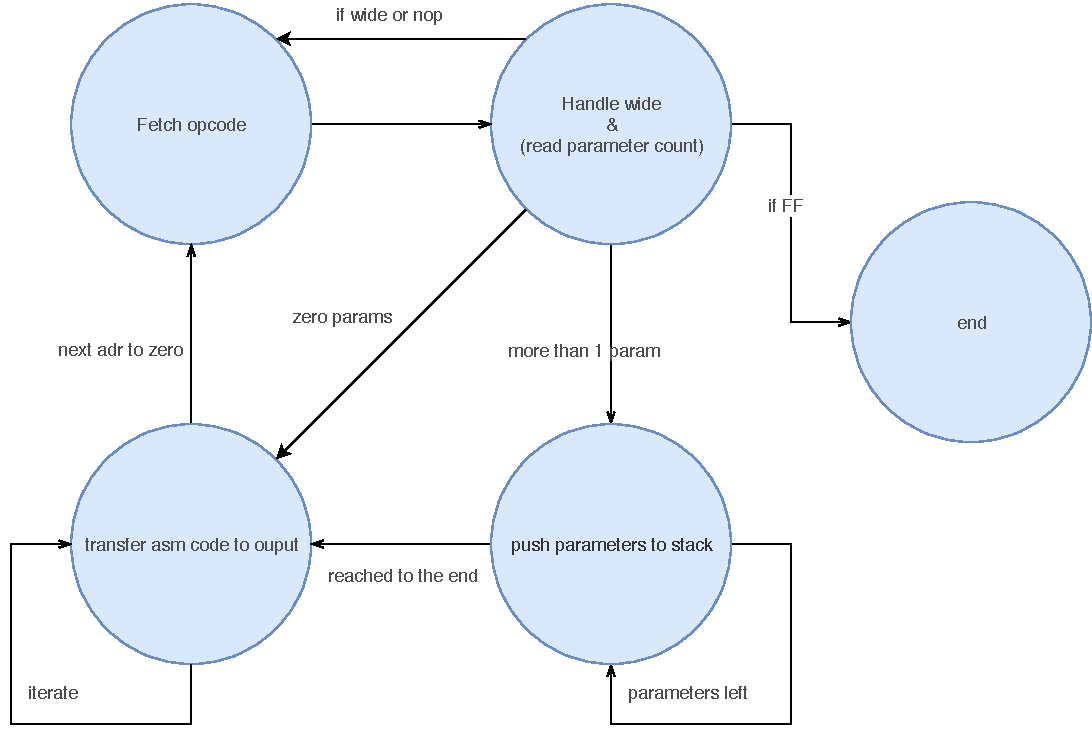
\includegraphics[width=0.9\linewidth]{SM}
	\caption{ماشین حالت}
	\label{fig:sm}
\end{figure}
%%% May add some information
\subsection*{\lr{FETCH\_INSTRUCTION}}
در این استیت، آپکد دستور 
\lr{JVM}،
 از رم مربوط به آن خوانده می‌شود. و بعد برای بررسی نوع دستور و گرفتن تعداد پارامترهای آن، به استیت (۲) می‌رویم. 

\subsection*{\lr{CHECK\_WIDE\_AND\_READ\_COUNTER}}

با بررسی آپکد دستور که در مرحله‌ی قبل خوانده‌ایم، در این‌جا با بررسی نوع دستور، به یکی از استیت‌های زیر می‌رویم:
\subsection*{\lr{END}}
برای پایان برنامه از یک بایت که در دستورات JVM نیست
\LTRfootnote{reserved word}
 مانند
\lr{0xFF}
استفاده کرده‌ایم. در صورتی که آپکد برابر این کلمه باشد، برنامه‌ی داخل رم JVM تمام شده‌است و کار این ماژول به پایان می‌رسد. 
\subsection*{ITERATE}
با استفاده از
\lr{count\_rom}
-که همان‌طور که قبلاً توضیح داده شده‌است، ماژولی است که با توجه به آپکد دستوراتِ
\lr{JVM}،
  تعداد بایت پارامترهایی که بعد از آن آپکد قرار می‌گیرند را مشخص می‌کند - می‌توان تعداد پارامترهای هر آپکد را در این‌جا داشت. بنابراین اگر پارامتری پس از این آپکد نداشته باشیم، مستقیماً به این استیت می‌رویم.
	
	\section*{
	تست‌بنچ‌های مربوط به ماژول‌های ساخته‌شده
}
در نهايت پس از ساخت تمامى اين ماژول‌ها تست‌بنچ‌هايى نوشتيم و به كمك آن‌ها، پيش از Integration از صحت عملكرد آ‌ن‌ها، اطمينان حاصل كرديم.
این تست‌بنچ‌ها شامل تست‌بنچ‌های زیر هستند:
\begin{itemize}
	\item \textbf{\lr{next\_byte\_gen\_tb}}:
	که از آن برای بررسی صحت ماژول‌های 
	\lr{memory\_r}
	و
	\lr{next\_byte\_gen}
	استفاده می‌کنیم.
	
	\item \textbf{\lr{read\_count\_tb}}:
	که از آن برای بررسی صحت ماژول‌های 
	\lr{read\_count}
	و
	\lr{countr\_rom}
	استفاده می‌کنیم.
	\item \textbf{\lr{write\_tb}}:
	که از آن برای بررسی صحت ماژول‌های 
	\lr{memory\_w}
و
	\lr{write}
	استفاده می‌کنیم.
\end{itemize}

	
	\section*{پیاده‌سازی دستورات پردازنده به‌کمک
	اسمبلی
	\lr{ARM}
}

در این مرحله تمامی دستورات پردازنده را با کمک زبان اسمبلی
\lr{ARM}
پیاده‌سازی کردیم. این دستورات شامل موارد زیر می‌شوند:

\subsection*{دستورات ستون دوم شامل کار با استک و اعداد صحیح}

برای پیاده‌سازی دستورات dup و مشابه آن‌ها تنها از دو دستور push و pop استفاده شده‌است. به این شکل که به‌ترتیب ذکرشده در مراجع، موارد مربوطه را push و pop می‌کنیم.

دستورات pop
\lr{pop}
و
\lr{pop2}
نیز با استفاده از یک خط دستور pop قابل پیاده‌سازی هستند و برای دستور swap نیز مشابه دستورات قبلی عمل می‌کنیم.

\subsection*{دستورات سه ستون دیگر شامل دستورات کار با float و double}

برای کار با اعداد 
\lr{floating point}
در اسمبلی
ARM دستورات مشخصی وجود دارد اما این دستورات توسط coprocessor اجرا می‌شوند. برای این که به coprocessor متصل شویم، از چند خط کد در ابتدای فایل 
\lr{.s}
ارسالی استفاده کرده‌ایم. این خطوط شامل فعال کردن مواردی مانند fpu و اتصال به coprocessor می‌شود.

\subsubsection*{چالش‌های اجرای کدهای اسمبلی نیازمند
\lr{fpu}}
در ابتدا می‌خواستیم شبیه‌سازی دستورات اسمبلی را به کمک
\lr{Keil}
 انجام‌دهیم، اما پس از اندکی تلاش مشاهده‌کردیم که پردازنده‌های دارای
\lr{fpu}،
 از خانواده‌یِ
\lr{cortex-m} 
هستند که تنها دستوراتِ
\lr{Thumb}
  را پشتیبانی می‌کنند اما ما می‌خواستیم که از دستورات ۳۲بیتیِ
\lr{ARM}
   در این پروژه بهره‌ببریم.
  .
  بنابراین تصمیم‌گرفتیم که در این بخش از نرم‌افزار
\lr{DS-5}
   استفاده‌کنیم. پس از نصب نرم‌افزار
\lr{DS-5}
 ابتدا سعی‌کردیم تا به کمک 
\lr{Fast Model}
    شبیه‌سازی را انجام دهیم و با جست‌وجو میان
\lr{Fast Model}ها
 متوجه‌شدیم که باید از پردازنده‌های خانواده‌ی
 \lr{Cortex-A}
 استفاده‌کنیم و در بین این پردازنده‌ها ، پردازنده‌ی
\lr{Cortex-A7}
 را انتخاب‌کردیم زیرا این پردازنده هم دارای
\lr{fpu}
 است و هم از دستورات ARM پشتیبانی می‌کند.

در کامپایلر مربوطه، تنظیمات را به گونه‌ای انجام دادیم تا به جای استفاده از عملیات اعشاری
\lr{soft-fp}ِ،
 از
\lr{hard-fp}
  استفاده‌کند که در این‌جا، به این مشکل برخوردیم که کد ما وارد 
\lr{Trap}های
\lr{CPU}
 می‌شد.

بنابراین پس از کمی جست‌وجو در منابع مختلف، متوجه‌شدیم که ابتدا باید
\lr{fpu}
 را فعال‌کنیم و بعد در ادامه به سراغ کدهای مربوطه برویم زیرا در غیر این صورت دچار مشکل خواهیم‌شد. لذا در ابتدای کدهای اسمبلی، کدی نوشتیم که
\lr{fpu}
  را فعال‌کند و به کمک آن کد، می‌توانستیم که دستورات مربوط به
\lr{fp}
 را اجرا کنیم.
 
 کد اسمبلی مذکور به شکل زیر است:
\begin{latin}
\begin{verbatim}
area start, code
export StartHere
StartHere
MRC p15, 0, r0, c1, c1, 2
ORR r0, r0, #2_11<<10 ; enable fpu
MCR p15, 0, r0, c1, c1, 2
LDR r0, =(0xF << 20)
MCR p15, 0, r0, c1, c0, 2
MOV r3, #0x40000000
VMSR FPEXC, r3
import __main
b __main
\end{verbatim}
\end{latin}
  
  حال در هر مرحله پس از اجرای هر قطعه کد مربوطه، برای بررسی درستی آن، ثبات‌ها را
\lr{pop}
   می‌کردیم و مشاهده می‌کردیم که آیا نتیجه دلخواه در درون آن‌ها ذخیره‌شده‌است یا خیر.
  

\subsubsection*{پیاده‌سازی دستورات}
حال به نحوه‌ی پیاده‌سازی دستورات این بخش می‌پردازیم:

\begin{itemize}
	
	\item\textbf{
	 دستورات 
	 \lr{fconst}
	 و
	 \lr{dconst}
}

برای پیاده‌سازی این دستورات تنها کافیست عدد مربوطه را به درون یک ثبات
\lr{mov}
 کرده و آن را به درون استک 
\lr{push}
 کنیم. توجه‌کنید که برای دستورات
\lr{floating point}
   پیش از هر دستور باید کاراکتر 
\lr{v}
 را قرار دهیم و برای اعداد
\lr{float}
   از 
   \lr{.f32}
    و برای اعداد 
\lr{double}
    از
\lr{f64.} 
    استفاده‌کنیم. نکته دیگر پیاده‌سازی این دستورات این است که مقدار صفر را نمی‌توانیم به درون یک ثبات مشخص
\lr{mov}کنیم 
      و برای این کار از عملیات
\lr{sub}
       و کم‌کردن مقدار یک ثبات از خودش برای تولید عدد صفر استفاده کرده‌ایم.
	
	\item \textbf{
		دستورات ضرب و جمع و تفریق و تقسیم
	}
	
	برای چنین عملیاتی در دستوراتی مانند dsub یا 
	\lr{fdiv}،
	ابتدا دو مقدار را از استک pop کرده و سپس عملیات مربوطه را انجام می‌دهیم و حاصل را به درون استک push می‌کنیم. این دستورات نکته خاصی ندارند و تمامی عملیات ضرب، جمع، تفریق یا تقسیم توسط coprocessor انجام می‌شوند.
	
	\item \textbf{
		دستورات مربوط به compare
	}
	
	برای 4 دستور مربوط به compare ابتدا دو عدد را با vpop از استک pop کرده و با vcmp مقایسه می‌کنیم. توجه کنید که باید به مقایسه‌کننده مخصوص دستورات
	\lr{floating point}
	متصل شویم و برای این کار از یک خط دستور زیر استفاده می‌شود.
	\begin{latin}
		\begin{verbatim}
		VMRS APSR_nzcv, FPSCR 
		\end{verbatim}
	\end{latin}
	
	پس از آن از سه بلوک مختلف استفاده می‌کنیم: بلوک
\lr{eq}،
 بلوک
 \lr{gt}
  و بلوک
\lr{lt}
 که هر یک شامل دو خط کد است و عملکرد برنامه را در صورت تساوی، بزرگ‌تر یا کوچک‌تر بودن مقایسه تعیین خواهد کرد.
	\item \textbf{
		دستورات load و store
	}
	
	در دستورات 
\lr{daload}
 و 
 \lr{faload}
  ابتدا دو عدد از استک می‌خوانیم که تعیین‌کننده محل خواندن از حافظه است. یکی از آن‌ها را به‌عنوان مبدا گرفته و دیگری را در 4 ضرب کرده و به آن می‌افزاییم تا محل خواندن عدد مربوطه به‌دست آید. سپس از محل به‌دست‌آمده در حافظه یکی از ثبات‌ها را
 \lr{load}کرده
  و حاصل را به درون استک 
\lr{push}می‌کنیم.
در دستورات
\lr{store}
 نیز کار مشابه است با این تفاوت که عددی که باید ذخیره‌شود را در ابتدا از استک خوانده و پس از آن دو عدد دیگر می‌خوانیم که به شکل ذکرشده در بالا، محل ذخیره‌سازی در حافظه را مشخص می‌کنند. در نهایت عددی که در ابتدای کار خوانده‌شد را در حافظه ذخیره می‌کنیم.
	
	\item\textbf{
		دستورات frem و fneg
	}
	
	دستور fneg بسیار ساده است. یک عدد را از درون استک pop کرده و با دستور
	\lr{vneg.f32}
	منفی کرده و در نهایت به‌درون استک push می‌کنیم. دستور frem نیز طبق فرمول ذکرشده در مراجع پیاده‌سازی شده‌است اما توجه کنید که هنگام انجام تقسیم اول که مربوط به اعداد
	\lr{floating point}
	است؛ باید حاصل را به یک integer تبدیل کنیم. برای این امر از دستور vcvt استفاده می‌کنیم که بعد از آن باید فرمت مبدا و فرمت مقصد را بنویسیم. برای مثال برای تبدیل حاصل
	\lr{floating point }
	تقسیم به عدد صحیح از دستور زیر بهره می‌گیریم که
	\lr{s32}
	نشان‌دهنده فرمت مقصد و
	\lr{f32}
	نشان‌دهنده فرمت مبدا خواهد بود.
	
	\begin{latin}
		\begin{verbatim}
		vcvt.s32.f32 s2,s2 
		\end{verbatim}
	\end{latin}
	
	\item \textbf{
		دستورات convert 
		ساده
	}
	
	دستوراتی مانند
	\lr{d2f}
	و
	\lr{f2i} 
	و 
	\lr{f2d}
	و
	\lr{d2i} 
	دستورات
	convert
	ساده هستند. 
	رای این دستورات تنها کافی‌ست از استک عدد مورد نظر را بخوانیم، به‌کمک دستور vcvt توضیح داده‌شده در بالا آن را به فرمت مورد نظر تبدیل کرده و در نهایت حاصل را به درون استک push کنیم.
	
	
	\item \textbf{
		دو دستور پیچیده تر convert
	}
	
	برای پیاده‌سازی دو دستور
	\lr{f2l}
	و
	\lr{d2l} 
	به این شکل عمل می‌کنیم که از دو خط کد آماده یافت‌شده در اینترنت برای انجام این تبدیل استفاده می‌کنیم که این دو خط کد به شکل زیر خواهد بود:
	
	
	\begin{latin}
		\begin{verbatim}
		import __aeabi_d2lz 
		bl __aeabi_d2lz
		\end{verbatim}
	\end{latin}
	
	بدیهی است که در دستورات مربوط به float به جای d از f استفاده می‌شود. سایر خطوط کد نیز نکته جدیدی ندارد.
	
	\item \textbf{
		دستورات fload
	}
	
	
	برای پیاده‌سازی دستور
	\lr{fload}،
	ابتدا یک عدد را از استک می‌خوانیم و به‌کمک شیفت چپ آن را در 4 ضرب می‌کنیم. سپس حاصل را با
	\lr{frame pointer}
	یا همان fp جمع‌کرده تا محل خواندن از حافظه به‌دست آید. سپس از محل مربوطه در حافظه خوانده و در یک ثبات ذخیره می‌کنیم و در نهایت حاصل را به درون استک، push می‌کنیم.
	
	برای دستورات
	\lr{fload\_n}
	نیز فرمت کلی زیر را داریم:
	
	\begin{latin}
		\begin{verbatim}
		vldr.f32 s0,[fp, #n*4] 
		vpush.f32 {s0}
		\end{verbatim}
	\end{latin}
	
	که به این معناست که از fp به اندازه 4 برابر n جلو می‌رویم و محتوا را از محل حافظه می‌خوانیم و در نهایت محتوای خوانده‌شده را به درون استک push می‌کنیم.
	
	\subsubsection*{اضافه‌کردن کدهای اسمبلی به 
		\lr{Instruction ROM}}
	
	حال دستورات پیاده‌سازی‌شده را هر یک به فرمت زیر می‌نویسیم:
	
	\begin{latin}
		\begin{verbatim}
		;#<instr_name> <ARM Code>
		\end{verbatim}
	\end{latin}
	
	و هدف این است که دستورات نوشته‌شده با این فرمت را به کد پایتونی که در بالا  ذکر شد بدهیم تا 
	\lr{Instruction ROM}
	را به صورت خودکار برای ما تولید کند.
\end{itemize}

\subsection*{کد پایتون و 
\lr{Assembler}
}
در کد پایتون ذکرشده،
 هر بار Assembler را صدا می‌کنیم و رشته‌های باینری مربوطه را به کمک اجرای Assembler از آن استخراج می‌کنیم تا برای ROM استفاده‌شود.

توجه‌کنید که در فاز نهایی پروژه کد پایتون مذکور را بهینه‌کرده‌ایم،سس بنابراین این کد علاوه بر این که محتوای
\lr{ROM}
 را همان‌طور که ذکر شد، تولید می‌کند؛ اگر هر کدی به آن به عنوان ورودی بدهیم، خیلی سریع کامپایل خواهد کرد و تست‌کیس مربوطه را برای ما تولید خواهدکرد. این بهینه‌سازی و فرآیند کامپایل سریع، سبب گرفتن خروجی در کمترین زمان ممکن خواهدشد و به‌وضوح کار بسیار مفیدی خواهد بود.
	
	\section*{سنتزکردن کدها}

پس از این که به کمک دستورات نوشته‌شده با اسمبلی 
\lr{ARM}
 و کد پایتون ذکرشده، 
\lr{ROM}ای 
که در قسمت‌های قبل توضیح‌داده‌شد را پرکردیم؛ مجموعه کدهای وریلاگمان کامل خواهدشد و حال باید این کدها را سنتزکنیم.

برای سنتز کدهای وریلاگ از نرم افزار
\lr{Quartus}
 محصول شرکت
\lr{Altera}
   استفاده‌کردیم و برای این کار در کوارتوس یک پروژه ساخته و تمامی فایل‌هایی که می‌خواهیم سنتزکنیم (تقریبا تمامی فایل‌ها به جز تست‌بنچ‌ها) را به آن پروژه اضافه‌نمودیم. 

سپس با چندین بار تلاش برای سنتز کدها ، اشکالات موجود و بخش‌های غیرِ سنتزپذیر کد را از آن حذف‌کردیم و با قطعه کدهای سنتزپذیر جایگزین‌کردیم تا در نهایت سنتز ماژول اصلی یعنی ماژول
\lr{top} 
 که در اصل مربوط به
\lr{Integration} 
  تمامی مواردی بود که پیاده‌سازی کرده‌ایم، انجام‌شد.

برای راحت‌ترشدن اجرا و تست و
\lr{import }کردن 
 فایل‌های سنتزشده به نرم‌افزار مادل‌سیم، از یک اسکریپت استفاده‌کردیم که با گرفتن ورودی، خود به خود نرم‌افزار مادل‌سیم را بازکرده و شبیه‌سازی را انجام‌داده و نتیجه را به ما ارائه می‌دهد. این اسکریپت سبب شد که سرعت تست کردن کدها و نتایج بسیار بالا رود و بتوانیم سریع‌تر مشکلات کدها را یافته و آن ها را برطرف کنیم.

در نهایت پس از رفع اشکالات کد مذکور، بالاخره خروجی تولیدشده توسط کد با خروجی مورد انتظار ما مشابه‌شد که شکل آن را در شکل
\ref{fig:result}
 می‌کنید.

\begin{figure}[H]
	\centering
	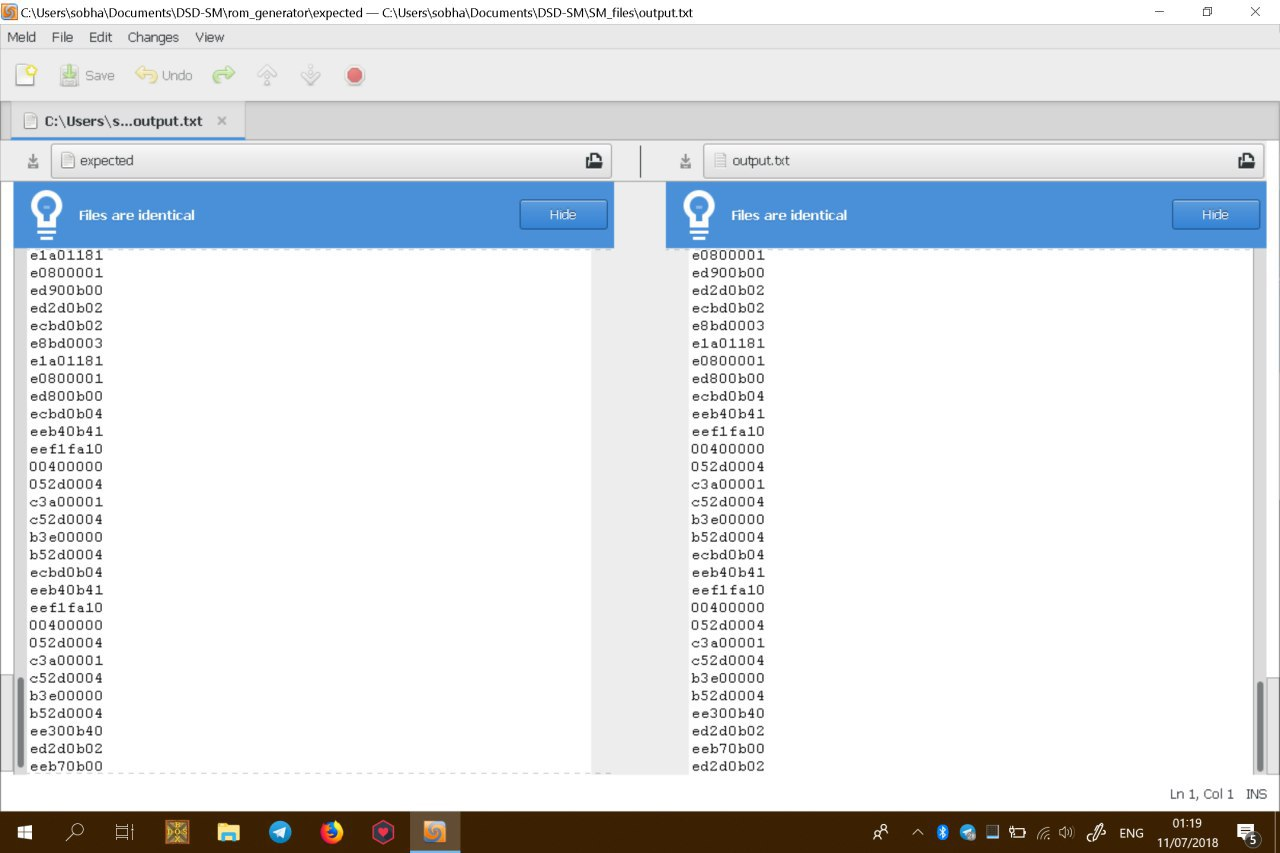
\includegraphics[width=0.8\linewidth]{result}
	\caption{نتیجه‌ی سنتز}
	\label{fig:result}
\end{figure}

	
	\section*{مراجع}
\begin{itemize}
	\item
	داک JVM در سایت ORACLE موجود در 
	\begin{latin}
	\href{https://docs.oracle.com/javase/specs/jvms/se7/html/index.html}{JSR-000924 Java® Virtual Machine Specification}
	\end{latin}
\end{itemize}
\end{document} 